\section{From a Link to a ZX-Diagram}\label{sec:passage}

We begin by describing the passage from a link $L$ to a ZX-diagram $D$ which represents the evaluation of the Jones polynomial of $L$ at lattice roots of unity. The majority of this journey is as detailed in \citep{jones_tensors}, though the final small step into the ZX-calculus is new. Since this section aims to be comprehensible to those with no background in topology or statistical mechanics, we leave most of the details to \citep{jones_tensors}. We introduce only as many terms as needed to describe the passage fully, keeping definitions simple and providing several figures. After this first jargon-heavy section, we will be working almost exclusively in a ZX setting.\newline

We will define an \textit{n-component link} $L$ to be a smooth embedding of $n$ disjoint circles in $\mathbb{R}^3$. A \textit{link diagram} for $L$ is a projection of the link onto some plane in $\mathbb{R}^3$ but with over- and undercrossing information retained. Thus a given link has infinitely many link diagrams. Intuitively, a link diagram is what one produces when one attempts to draw a link in two dimensions. An \textit{oriented link} has a direction assigned to each component; this is indicated in a link diagram by an arrow. As an example is shown below:\newline

[diagram]\newline

Two oriented links $L$ and $L'$ are isotopic, written $L \simeq L'$, if and only if there is a finite sequence of \textit{Reidemeister moves} [ToDo: ref] taking a diagram for $L$ to a diagram for $L'$. These moves precisely capture the notion of reversible local strand deformations that do not change the topology. For example, they do not permit breaking or gluing of strands, passing one strand through another, or reversing of orientations. The \textit{Jones polynomial} $V_L(z)$ for an oriented link $L$ is a polynomial in $z \in \mathbb{C}$. It is a \textit{link invariant}; that is, $V_L(z) \neq V_{L'}(z)$ implies $L \not\simeq L'$, for any two oriented links $L$ and $L'$. In general, computing $V_L(z)$ is exponentially costly in the number $\abs{C}$ of crossings of $L$, but it is known that at the special cases of the \textit{lattice roots of unity} $z \in \{\pm 1, \pm i, \pm e^{i\frac{2\pi}{3}}, \pm e^{i\frac{4\pi}{3}}\}$ it can be evaluated in time polynomial in $\abs{C}$ [Welsh]:\newline

[Draw lattice roots of unity]\newline

Now, for any diagram of a link $L$ there is an associated \textit{Tait graph}. This is denoted $G_L = (V_L, E_L)$ and obtained as follows. First, the link diagram is given a \textit{checkerboard colouring}. That is, regions of $\mathbb{R}^2$ carved out by the link are shaded black or white such that no two adjacent regions have the same colour. For any diagram for $L$ there are exactly two equivalent ways to do this, the difference between the two just being that the roles of black and white are swapped throughout. Therefore we fix a convention that the unique unbounded region surrounding the link (i.e. the background) will be white.\newline

[diagram]\newline

Next, every shaded (black) region is mapped to a vertex and every crossing is mapped to a signed edge $e = vw$ according the rule shown below. The signs $\varepsilon_{vw} = \pm$ of these edges are called \textit{Tait signs} and are graphically denoted by a small box on the corresponding edge, labelled with either a plus or minus sign appropriately:\newline

[diagram]\newline

If we now suppose that the vertices and Tait signs actually represent \textit{tensors} (multidimensional matrices), then this Tait graph above can be interpreted as a closed \textit{tensor network} in diagrammatic notation [ToDo: ref], which we'll denote $Z(q)$. In fact, suppose we let $z_q = \frac{1}{2}\left(q - 2 + \sqrt{q(q - 4)}\right)$, and let the vertices and Tait signs denote the following tensors:

\begingroup
	\renewcommand*{\arraystretch}{1.25}
	\begin{equation}\label{eq:pm_tensor}
		T_\pm^{(q)} = 
		\left\llbracket \ \tikzfig{pm_maps/pm} \ \right\rrbracket = 
		\begin{pmatrix}
			-z_q^{\mp 1} & 1 & \dots & 1 \\
			1 & -z_q^{\mp 1} & \dots & 1 \\
			\vdots & \vdots & \ddots & \vdots\\
			1 & 1 & \dots & -z_q^{\mp 1}
		\end{pmatrix}
	\end{equation}
	\begin{equation}\label{eq:vertex_tensor}
		\tilde{T}^{(q)} =
		\left\llbracket \ \ \tikzfig{pm_maps/vertex} \ \ \right\rrbracket = 
		\text{ToDo}
	\end{equation}
\endgroup

Then remarkably the resulting closed tensor network $Z(q)$ is equal to the Jones polynomial $V_L(z_q)$ at these specific points, up to a prefactor $\mathcal{A}_L(q)$ [ToDo: ref]. Computing this prefactor is known to be efficient, so if we can show that computing $Z(q)$ is also efficient then we'll have shown that computing $V_L(z_q)$ is efficient. Note the correspondence $(z_1, z_2, z_3, z_4) = (e^{i\frac{2\pi}{3}}, i, e^{i\frac{\pi}{3}}, 1)$ with the lattice roots of unity. 

\begin{remark}
	Of course, different diagrams for $L$ will lead to different (non-isomorphic) Tait graphs $G_L$. Ultimately, however, this will not matter to us. This is because the Tait signs $\varepsilon_{vw}$ are related to $z_q$ in such a way that graph operations on $G_L$ corresponding to Reidemeister moves on $L$ leave $Z(q)$ (ToDo: and $\mathcal{A}_L(q)$?) invariant [ToDo: ref].
\end{remark}

\begin{remark}
	$Z(q)$ is in fact the partition function of a $q$-state Potts model placed on the Tait graph $G_L$. [ToDo: say more?]
\end{remark}

In order to demonstrate efficient computability of $Z(q)$ for $q \in \{1, 2, 3, 4\}$, we will find representations for the tensors $T_\pm^{(q)}$ and $\tilde{T}^{(q)}$ in the \textit{ZX-calculus}, a graphical language for quantum mechanics based on $q$-dimensional qudits, introduced formally in the next two sections. For $q=1$ the calculus is trivial - there is exactly one $1$-dimensional qudit - so only the cases $q \in \{2, 3, 4\}$ remain. For $q=4$ the isomorphism $\mathbb{C}^4 \cong \mathbb{C}^2 \otimes \mathbb{C}^2$ means we can use the same 2-dimensional calculus as for $q=2$. We will soon see that both the 2-dimensional (\textit{qubit}) and 3-dimensional (\textit{qutrit}) ZX-calculus feature \textit{green spiders}, and in all three cases $q \in \{2, 3, 4\}$ these are the right choice of representative of the vertex tensor $\tilde{T}^{(q)}$.

\begin{proposition}\label{prop:vertex_tensor_Z_spider}
	The tensor represented by a vertex in the Tait graph is related (ToDo: how!?) to the \textit{standard interpretation} of the green spider in the cases $q \in \{2, 3, 4\}$.
	\begin{equation*}
		\tilde{T}^{(q)} \ = \ 
		\left\llbracket \ \ \tikzfig{pm_maps/vertex} \ \ \right\rrbracket \ \sim \ 
		\left\llbracket \ \ \tikzfig{pm_maps/z_spider} \ \ \right\rrbracket
	\end{equation*}
	\begin{proof}
		See Appendix [ToDo].
	\end{proof}
\end{proposition}

ZX-diagrams corresponding to the $q \times q$ matrix $T_\pm^{(q)}$ are given after the ZX-calculi have been properly introduced (Propositions \ref{prop:pm_map_q2_q4} and \ref{prop:pm_map_q3}). [ToDo: say more! Move discussion about scalar exactness here? Explain how contracting this tensor network/ZX-diagram means evaluating $Z(q)$?]


% Let $z_q = \frac{1}{2}\left(q - 2 + \sqrt{q(q - 4)}\right)$, and note the correspondence $(z_1, z_2, z_3, z_4) = (e^{i\frac{2\pi}{3}}, i, e^{i\frac{\pi}{3}}, 1)$ with the lattice roots of unity. Remarkably, the Jones polynomial $V_L(z_q)$ at the points $q \in \{1, 2, 3, 4\}$ can be expressed in terms of the \textit{partition function} $Z(q)$ of a \textit{$q$-state Potts model} [Wu]. 



% For those with no statistical mechanical background, given some graph $G = (V, E)$, a $q$-state Potts model on $G$ can just be thought of as the ability to assign a \textit{spin} $\sigma_v \in \{1, ..., q\}$ to each vertex $v \in V$, along with a partition function $Z: \{1, .., q\} \rightarrow \mathbb{C}$, which in physics usually captures some thermodynamical properties of a system. This function has an explicit formula in the general case, but it will make more sense to defer stating this until we have introduced enough terminology to give a simpler formula pertaining to our circumstances (see [ToDo] below). A particular assignment $\sigma = (\sigma_1, ..., \sigma_{\abs{V}})$ of spins to each vertex will be called a \textit{configuration}.\newline

% In our case, we will define a Potts model on a particular \textit{signed graph} - a graph in which every edge has a positive or negative sign - called a \textit{Tait graph} of the link $L$. This is denoted $G_L = (V_L, E_L)$ and obtained as follows. First, an arbitrary link diagram for $L$ is given a \textit{checkerboard colouring}. That is, regions of $\mathbb{R}^2$ carved out by the link are shaded black or white such that no two adjacent regions have the same colour. For any diagram for $L$ there are exactly two equivalent ways to do this, the difference between the two just being that the roles of black and white are swapped throughout. Therefore we fix a convention that the unique unbounded region surrounding the link (i.e. the background) will be white.\newline

% [Diagram]\newline

% Next, every shaded (black) region is mapped to a vertex and every crossing is mapped to a signed edge $e = vw$ according to its orientation relative to the surrounding colours, per the rule shown in [ToDo] below. The signs $\varepsilon_{vw} = \pm$ of these edges are called \textit{Tait signs} and are graphically denoted by a small box on the corresponding edge, labelled with either a plus or minus sign appropriately. If we now define a Potts model on $G_L$, the partition function $Z(q)$ has the following formula. We sum over all possible configurations $\sigma$ of spins, and within each term we multiply together the values $-z_q^{-\varepsilon_{vw}}$ for all edges $vw$ whose endpoints have the same spin in this configuration. That is:

% \begin{equation}
% 	Z(q) = \sum_{\sigma} \left( \prod_{vw \in E_L} T_{\sigma_v, \sigma_w}^{(q)} \right)
% \end{equation}
% \begin{equation}
% 	T_{\sigma_v, \sigma_{w}}^{(q)}
% 	= \begin{cases}
% 		-z_q^{-\varepsilon_{vw}} &\ \ \text{if} \ \ \sigma_v = \sigma_{w} \\  
% 		1 &\ \ \text{if} \ \ \sigma_v \neq \sigma_{w}
% 	\end{cases}
% \end{equation}

% For fixed $v, w$ we can view $T_{(-)_v,(-)_w}^{(q)} \eqdef T_{\varepsilon_{vw}}^{(q)}$ as a $q \times q$ matrix, indexed by the possible spins $\{1, ..., q\}$ that could be assigned to $v$ and $w$: 

% \begingroup
% 	\renewcommand*{\arraystretch}{1.5}
% 	\begin{equation}
% 	T_{-_v,-_w}^{(q)}
% 	\begin{pmatrix}
% 		-z_q^{-\varepsilon_{vw}} & 1 & \dots & 1 \\
% 		1 & -z_q^{-\varepsilon_{vw}} & \dots & 1 \\
% 		\vdots & \vdots & \ddots & \vdots\\
% 		1 & 1  & \dots & -z_q^{-\varepsilon_{vw}}
% 	\end{pmatrix}
% \end{equation}
% \endgroup

% Finally, the actual statement relating the Jones polynomial to the partition function is:

% \begin{equation}
% 	V_L(z_q) = \mathcal{A}_L(q)Z(q)
% \end{equation}

% where $\mathcal{A}_L(q)$ is an efficiently computable prefactor, whose definition is given in Appendix [ToDo]. 
% % For completeness, we give its formula, where $w(L)$ denotes the \textit{writhe} of the link $L$ [ToDo: ref], and the \textit{Tait number} $\tau(L)$ is the sum $\sum_{vw \in E_L} \varepsilon_{vw}$ of all the Tait signs:
% % \begin{equation}
% % 	\mathcal{A}_L(q) = (-z_q^{\frac{1}{2}} - z_q^{-\frac{1}{2}})^{-\abs{V_L} - 1}(-z_q^{\frac{3}{4}})^{w(L)}z_q^{\frac{1}{4}\tau(L)}
% % \end{equation}

% \begin{remark}
% 	Of course, different diagrams for $L$ will lead to different (non-isomorphic) Tait graphs $G_L$. Ultimately, however, this will not matter to us. This is because the Tait signs are related to $z_q$ in such a way that graph operations on $G_L$ corresponding to Reidemeister moves on $L$ leave $Z(q)$ (ToDo: and therefore $\mathcal{A}_L(q)$?) invariant [ToDo: ref].
% 	 % $\varepsilon_{vw} = \pm$ determine \textit{spin-spin interactions} $J_{\pm} = \text{[ToDo]}$, which are related to the variable $z_q$ of the Jones polynomial $V_L(z_q)$ via the equality $z_q = -e^{\mp J_\pm}$. As a result, it can be shown [ToDo ref] that the interactions $J_\pm$ are such that the graph operations on $G_L$ corresponding to Reidemeister moves on $L$ leave $Z(q)$ invariant. 
% \end{remark}



% After defining a Potts model on the Tait graph $G_L$, every signed edge indicates a \textit{spin-spin Tait-sign-dependent interaction} $J_\pm \in \mathbb{C}$. These interactions relate to the variable $z$ of the Jones polynomial via the equality $z = -e^{\mp J_\pm}$. The role of the link invariant is played by the partition function $Z(q)$; in fact, the interactions $J_\pm$ are such that the graph operations on $G_L$ corresponding to Reidemeister moves on $L$ leave $Z(q)$ invariant. Specifically, $Z(q)$ is related to the Jones polynomial by $V_L(z) = \mathcal{A}_L(z)Z(q)$, where $A_L(z)$ is an efficiently computable value which handles bookeeping of twist factors [Definition?]. Its explicit definition is given in [ToDo] in the Appendix. has the following explicit formula: [Check again with Kon!]\newline






% For the case $q=3$ we use the qutrit ZX calculus:
% % \begin{equation}
% % 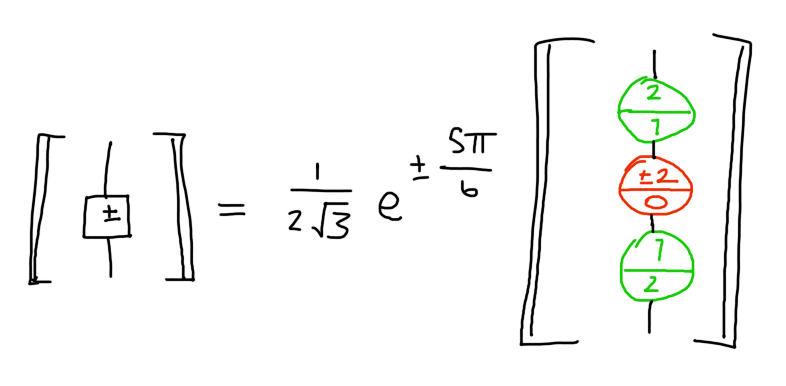
\includegraphics[scale=0.3]{figures/sketches/Qutrit Potts matrices.png}
% % \end{equation}

% For the case $q=4$ we are back again in the usual qubit ZX calculus:
% % \begin{equation}
% % 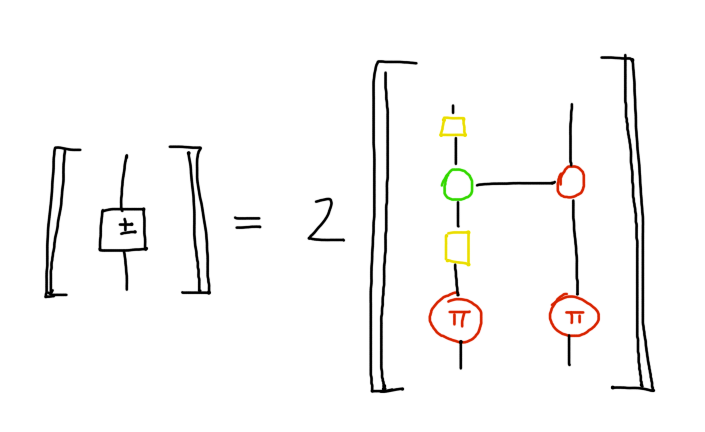
\includegraphics[scale=0.3]{figures/sketches/Qu(4)it Potts matrices.png}
% % \end{equation}

% In each case, the resulting map is in the stabilizer fragment of the ZX calculus. 
